% Figure 1: Delta Accumulator Architecture
% 
% This file contains TikZ code for the delta accumulator diagram.
% Can be compiled standalone or included in main.tex
%
% SPECIFICATION:
% - Show multiple input deltas (δ₁, δ₂, δ₃, ..., δₙ) entering from left
% - XOR tree in the middle reducing deltas in parallel
% - Single accumulated delta (δₐcc) output from tree
% - Final XOR with initial state (S₀) to produce final state (S')
% - Timing annotations showing O(log n) for tree, O(1) for final XOR
% - Color coding: inputs (blue), XOR operations (orange), outputs (green)

\documentclass[tikz,border=10pt]{standalone}
\usepackage{tikz}
\usetikzlibrary{arrows.meta,shapes,positioning,calc,decorations.pathreplacing}

\begin{document}
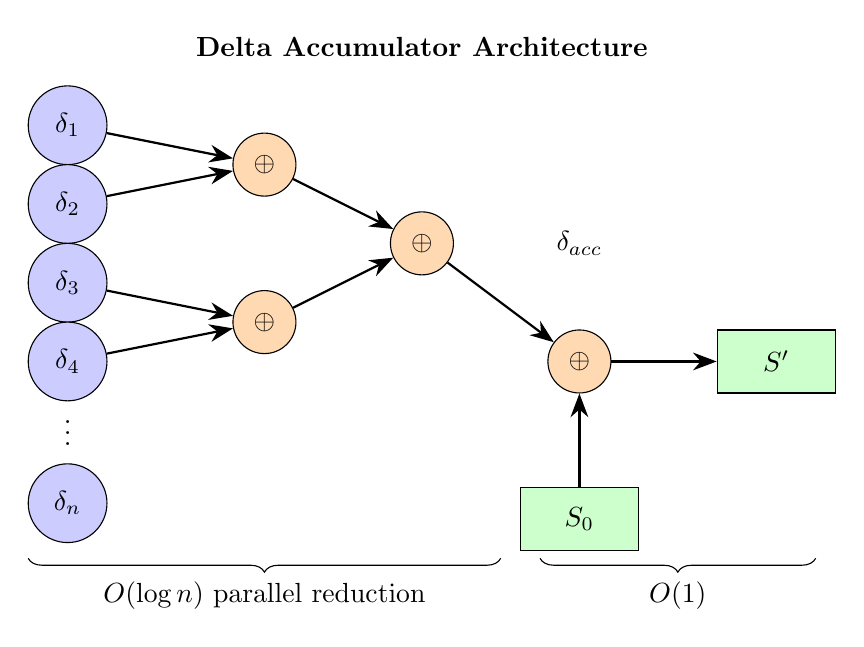
\begin{tikzpicture}[
    delta/.style={draw, circle, minimum size=1cm, fill=blue!20},
    xor/.style={draw, circle, minimum size=0.8cm, fill=orange!30},
    state/.style={draw, rectangle, minimum width=1.5cm, minimum height=0.8cm, fill=green!20},
    arrow/.style={-{Stealth[length=3mm]}, thick}
]

% Input deltas
\node[delta] (d1) at (0, 3) {$\delta_1$};
\node[delta] (d2) at (0, 2) {$\delta_2$};
\node[delta] (d3) at (0, 1) {$\delta_3$};
\node[delta] (d4) at (0, 0) {$\delta_4$};
\node at (0, -0.8) {$\vdots$};
\node[delta] (dn) at (0, -1.8) {$\delta_n$};

% First level XOR
\node[xor] (x1) at (2.5, 2.5) {$\oplus$};
\node[xor] (x2) at (2.5, 0.5) {$\oplus$};

% Second level XOR
\node[xor] (x3) at (4.5, 1.5) {$\oplus$};

% Final accumulator output
\node[xor] (xacc) at (6.5, 0) {$\oplus$};

% Initial state
\node[state] (s0) at (6.5, -2) {$S_0$};

% Final state
\node[state] (sf) at (9, 0) {$S'$};

% Accumulated delta label
\node at (6.5, 1.5) {$\delta_{acc}$};

% Arrows
\draw[arrow] (d1) -- (x1);
\draw[arrow] (d2) -- (x1);
\draw[arrow] (d3) -- (x2);
\draw[arrow] (d4) -- (x2);

\draw[arrow] (x1) -- (x3);
\draw[arrow] (x2) -- (x3);

\draw[arrow] (x3) -- (xacc);
\draw[arrow] (s0) -- (xacc);
\draw[arrow] (xacc) -- (sf);

% Timing annotations
\draw[decorate, decoration={brace, amplitude=5pt, mirror}] 
    (-0.5, -2.5) -- (5.5, -2.5) node[midway, below=5pt] {$O(\log n)$ parallel reduction};
\draw[decorate, decoration={brace, amplitude=5pt, mirror}] 
    (6, -2.5) -- (9.5, -2.5) node[midway, below=5pt] {$O(1)$};

% Title
\node at (4.5, 4) {\textbf{Delta Accumulator Architecture}};

\end{tikzpicture}
\end{document}
